\documentclass{standalone}
\usepackage{tikz}
\usetikzlibrary{positioning}

\begin{document}

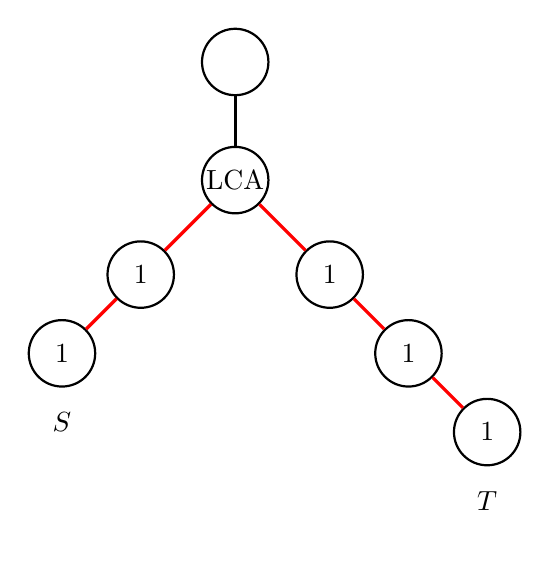
\begin{tikzpicture}[every node/.style={circle,draw,minimum size=24pt,inner sep=0pt},thick]

% 节点
\node (lca) at (0,0) {LCA};
\node (up) at (0,1.5) {~}; % Use ~ to maintain node size
\node (a1) at (-1.2,-1.2) {1};
\node (a2) at (1.2,-1.2) {1};
\node (s1) at (-2.2,-2.2) [label=below:$S$] {1};
\node (a3) at (2.2,-2.2) {1};
\node (t1) at (3.2,-3.2) [label=below:$T$] {1};

% 连线
\draw[black,very thick] (lca) -- (up);
\draw[red,very thick] (lca) -- (a1);
\draw[red,very thick] (lca) -- (a2);
\draw[red,very thick] (a1) -- (s1);
\draw[red,very thick] (a2) -- (a3);
\draw[red,very thick] (a3) -- (t1);

\end{tikzpicture}

\end{document}